%! Author = admin
%! Date = 2023/12/17

% Preamble
\documentclass[a4paper]{article}

% Packages
\usepackage[margin=1in]{geometry}
\usepackage[fontset=founder]{ctex}
\usepackage{anyfontsize}
\usepackage{graphicx,caption,subcaption}
\usepackage{amsmath,amssymb,mathabx}
\usepackage{multirow}
\usepackage{algorithm,algorithmicx,algpseudocode}
\usepackage{hyperref}
\usepackage{listings}
\usepackage[usenames,dvipsnames]{xcolor}

\graphicspath{{../figures/}}

\definecolor{mygreen}{rgb}{0,0.6,0}
\definecolor{mygray}{rgb}{0.5,0.5,0.5}
\definecolor{mymauve}{rgb}{0.58,0,0.82}
\lstset{
    backgroundcolor=\color{white},
    basicstyle = \footnotesize,
    breakatwhitespace = false,
    breaklines = true,
    captionpos = b,
    commentstyle = \color{mygreen}\bfseries,
    extendedchars = false,
    frame =shadowbox,
    framerule=0.5pt,
    keepspaces=true,
    keywordstyle=\color{blue}\bfseries, % keyword style
    language = C++,                     % the language of code
    otherkeywords={string},
    numbers=left,
    numbersep=5pt,
    numberstyle=\tiny\color{mygray},
    rulecolor=\color{black},
    showspaces=false,
    showstringspaces=false,
    showtabs=false,
    stepnumber=1,
    stringstyle=\color{mymauve},        % string literal style
    tabsize=2,
    title=\lstname
}

\renewcommand{\algorithmicrequire}{\textbf{Input:}}
\renewcommand{\algorithmicensure}{\textbf{Output:}}

\title{\textbf{数据结构实验报告}}
\author{姚苏航\qquad PB22061220}
\date{}


% Document
\begin{document}
    \maketitle


    \section{问题描述}\label{sec:des}

    \subsection{实验题目}\label{subsec:q}
    {{利用哈希表统计两源程序的相似性。}}

    \subsection{基本要求}\label{subsec:req}
    {{对于两个C语言的源程序清单,
    用哈希表的方法分别统计两程序中使用C语言关键字的情况,
    并最终按定量的计算结果,得出两份源程序的相似性。}}

    \subsection{测试数据}\label{subsec:test}
    {{事先给出的file文件夹,包含关键词表和三份源程序文件,程序之间有相近的和差别大的。
    文件内容详见附录~\ref{sec:appendix2}。}}


    \section{需求分析}\label{sec:need}

    \noindent{1.扫描给定的源程序,累计在每个源程序中 C 语言关键字出现的频度
        (为保证查找效率,建议自建哈希表的平均查找长度不大于2),
        通过这种方式扫描两个源程序,提取其特征向量。}

    \noindent{2.通过计算向量Xi和Xj的相似值来判断对应两个程序的相似性,
    相似值的判别函数计算公式为:}
    \begin{equation}
        S(X_i,X_j)=\frac{X_i^T\cdot X_j}{|X_i|\cdot|X_j|}\label{eq:equation}
    \end{equation}
    \noindent{\;\;\,\ 通过这种方式,可以初步判断两个源程序的相似性,
    如图1所示。其中 S 反映了两向量的夹角的余弦,当 S 趋近于 1 时,
    两向量夹角趋于 0 ,即两向量趋于相似,反之亦然。}
    \begin{figure}[htbp]
        \centering
        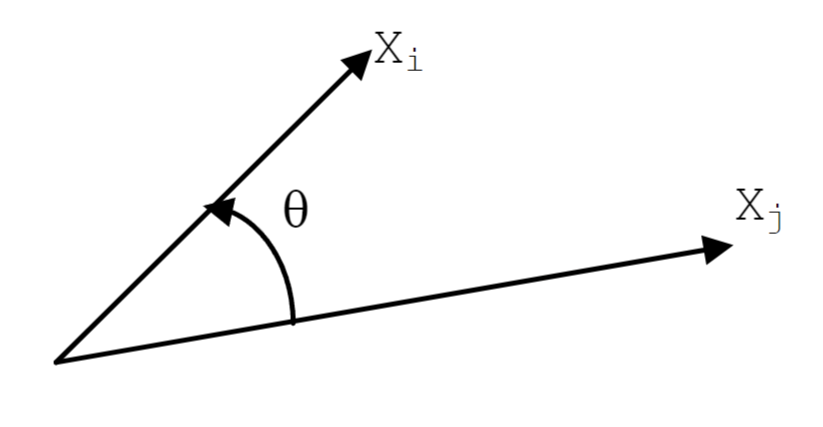
\includegraphics[height=120pt]{S}
        \caption{Similarity}\label{fig:figure}
    \end{figure}

    \noindent{3.在有些情况下,S 不能很好地反映两向量的相似性,还需要进一步的考虑。
    例如,在 S 接近于 1 时,两向量的模的差距不能很好地被反映,如图2所示。
    因此引入几何距离 D ,用于反应两向量终点间的距离。}
    \begin{figure}[htbp]
        \centering
        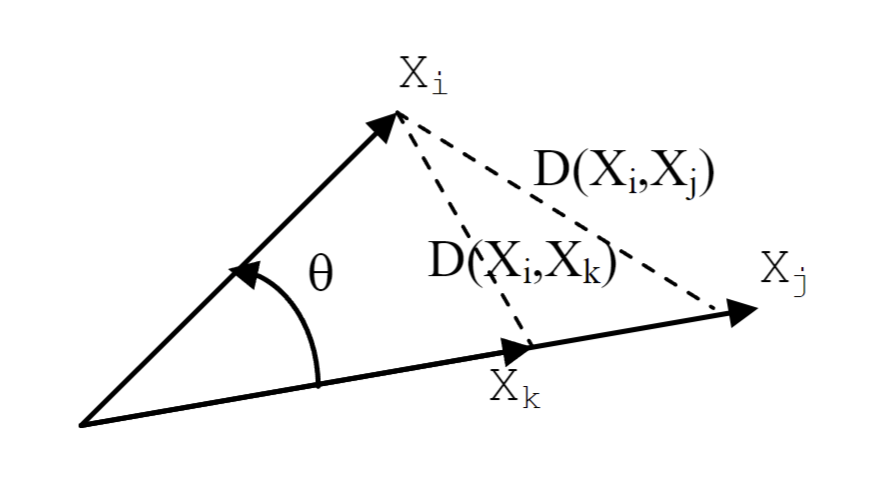
\includegraphics[height=120pt]{D}
        \caption{Distance}\label{fig:figure2}
    \end{figure}

    \noindent{4.通过分别比较很相近和差别很大的三个源代码,实践这种方法的有效性。}


    \section{概要设计}\label{sec:design1}

    \subsection{所用到得数据结构及其ADT}\label{subsec:adt}
    \begin{algorithm}
        \caption{用归并排序求逆序数}
        \begin{algorithmic}[1] %每行显示行号
            \Function {MergerSort}{$Array, left, right$}
                \State $result \gets 0$
                \If {$left < right$}
                    \State $middle \gets (left + right) / 2$
                    \State $result \gets result +$ \Call{MergerSort}{$Array, left, middle$}
                    \State $result \gets result +$ \Call{MergerSort}{$Array, middle, right$}
                    \State $result \gets result +$ \Call{Merger}{$Array,left,middle,right$}
                \EndIf
                \State \Return{$result$}
            \EndFunction
        \end{algorithmic}\label{alg:algorithm}
    \end{algorithm}

    \subsection{主程序流程及其模块调用关系}\label{subsec:relate}


    \section{详细设计}\label{sec:design2}

    \subsection{实现概要设计中的数据结构ADT}\label{subsec:adt2}
    \begin{lstlisting}[caption={},label={lst:lstlisting}]
        typedef struct {
            KeyType key;
            Datatype Data;  // 记录关键字出现的次数
        } ElemType;       // 包含关键字和数据

        typedef struct LHNode {  // 哈希表结点
            ElemType data;         // 查找表单元
            LHNode *next;          // 后继
        } *LHptr;

        typedef struct {
            LHptr *elem;
            int count;   // 记录数
        int size;    // 容量
        } LHashTable;  // 链地址存储法
    \end{lstlisting}

    \subsection{实现每个操作的伪码,重点语句加注释}\label{subsec:explain}

    \subsection{主程序和其他模块的伪码}\label{subsec:code2}


    \section{调试分析}\label{sec:debug}

    \subsection{问题分析与体会}\label{subsec:analysis}

    \subsection{时空复杂度分析}\label{subsec:analysis2}


    \section{使用说明}\label{sec:instrut}
    {{用户将事先准备好的关键词表(keyword.txt)和需要统计相似性的程序放入file文件夹中,
    运行时程序将通过关键词表建立哈希表,并通过查找哈希表构建两程序的向量,
    最后通过判别函数计算两程序相似性和向量的几何距离。}}

    {{在本项目中,使用事先给出的测试数据,
    准备三个编译和运行都无误的C程序,程序之间有相近的和差别大的,
    通过similar.c和different.c两个程序与main.c进行比较,
    可以直观展现出比较的效果。}}


    \section{测试结果}\label{sec:result}

    \subsection{输入数据}\label{subsec:in}
    {{输入数据从给出的测试文件中读取,
    读取keyword.txt文件生成哈希表,
    再分别读取main.c,similar.c,different.c并进行比较。}}

    \subsection{输出数据}\label{subsec:out}
    \noindent{输出结果显示在终端,内容如下:}

    \noindent{X\_(../file/similar.c):}

    \noindent{0 1 1 4 0 1 0 3 3 1 2 1 2 0 1 1 4}

    \noindent{X\_(../file/different.c):}

    \noindent{0 1 0 1 0 0 1 2 1 0 3 0 0 0 1 3 2}

    \noindent{X\_(../file/main.c):}

    \noindent{0 1 1 3 0 1 0 3 2 1 2 1 2 0 1 1 4}

    \noindent{ }

    \noindent{S\_(Sim\&Main):0.988174}

    \noindent{D\_(Sim\&Main):1.41421}

    \noindent{ }

    \noindent{S\_(Dif\&Main):0.740121}

    \noindent{D\_(Dif\&Main):4.89898}


    \appendix


    \section{实验源代码文件}\label{sec:appendix1}
    {{为方便查看,附录中的链接文件均为txt格式}}

    \href{../exp6/define.h.txt}{\underline{define.h}}

    \href{../exp6/main.cpp.txt}{\underline{main.cpp}}

    \href{../exp6/OpenHashing.h.txt}{\underline{OpenHashing.h}}

    \href{../exp6/OpenHashing.cpp.txt}{\underline{OpenHashing.cpp}}

    \href{../exp6/system.h.txt}{\underline{system.h}}

    \href{../exp6/system.cpp.txt}{\underline{system.cpp}}

    \href{../exp6/SimAsses.h.txt}{\underline{SimAsses.h}}

    \href{../exp6/SimAsses.cpp.txt}{\underline{SimAsses.cpp}}


    \section{实验用测试文件}\label{sec:appendix2}
    \href{../exp6/file/main.c.txt}{\underline{main.c}}

    \href{../exp6/file/different.c.txt}{\underline{different.c}}

    \href{../exp6/file/similar.c.txt}{\underline{similar.c}}

    \href{../exp6/file/keyword.txt}{\underline{keyword.txt}}


\end{document}


%    \begin{algorithm}
%        \caption{开散列哈希表}
%        \begin{algorithmic}[1] %每行显示行号
%            \Require $Array$数组,$n$数组大小
%            \Ensure 逆序数
%            \Function {MergerSort}{$Array, left, right$}
%                \State $result \gets 0$
%                \If {$left < right$}
%                    \State $middle \gets (left + right) / 2$
%                    \State $result \gets result +$ \Call{MergerSort}{$Array, left, middle$}
%                    \State $result \gets result +$ \Call{MergerSort}{$Array, middle, right$}
%                    \State $result \gets result +$ \Call{Merger}{$Array,left,middle,right$}
%                \EndIf
%                \State \Return{$result$}
%            \EndFunction
%            \State
%            \Function{Merger}{$Array, left, middle, right$}
%                \State $i\gets left$
%                \State $j\gets middle$
%                \State $k\gets 0$
%                \State $result \gets 0$
%                \While{$i<middle$ \textbf{and} $j<right$}
%                    \If{$Array[i]<Array[j]$}
%                        \State $B[k++]\gets Array[i++]$
%                    \Else
%                        \State $B[k++] \gets Array[j++]$
%                        \State $result \gets result + (middle - i)$
%                    \EndIf
%                \EndWhile
%                \While{$i<middle$}
%                    \State $B[k++] \gets Array[i++]$
%                \EndWhile
%                \While{$j<right$}
%                    \State $B[k++] \gets Array[j++]$
%                \EndWhile
%                \For{$i = 0 \to k-1$}
%                    \State $Array[left + i] \gets B[i]$
%                \EndFor
%                \State \Return{$result$}
%            \EndFunction
%        \end{algorithmic}\label{alg:algorithm2}
%    \end{algorithm}
